\documentclass{article}
\usepackage{graphicx}
\usepackage{hyperref}
\usepackage{array}
\usepackage{listingsutf8}
\usepackage{xcolor}

\author{Francesco Mauro}
\date{2023}
\title{Relazione Metodologie e Tecnologie didattiche per l'informatica}


\lstset{
  language=Go,
  basicstyle=\scriptsize\ttfamily,
  keywordstyle=\color{blue}\bfseries,
  commentstyle=\color{green},
  stringstyle=\color{red},
  breaklines=true,
  showstringspaces=false,
  numbers=left,
  numberstyle=\small,
  numbersep=5pt,
  backgroundcolor=\color{white},
  tabsize=2,
  morekeywords={package, import, func, var, const},
}



\begin{document}
\maketitle
\tableofcontents
\section{Motivazione e Finalità}

Attraverso la GUI vs CLI si può spiegare la differenza tra un programma strutturato con un'interfaccia da linea di comando oppure con una grafica. Ognuna delle due ha aspetti positivi e  negativi. Attraverso questa attività didattica lo studente dovrebbe comprendere meglio le differenze tra le due, e imparare a capire quando conviene usare un'interfaccia piuttosto che un'altra.

Un'ottima sintesi di definizione di CLI la si può trovare sul sito di Golang:
\begin{quote}
    
Command line interfaces (CLIs), unlike graphical user interfaces (GUIs), are text-only. Cloud and infrastructure applications are primarily CLI-based due to their easy automation and remote capabilities. 

\end{quote}

\section{Prerequisiti}
Lo studente dovrebbe avere delle basi di programmazione,come la conoscenza della differenza tra input e output e del concetto di libreria software, infine una conoscenza di  base di matematica; questa non è strettamente necessaria all'attività didattica ma per svolgere in maniera più semplice l'esercizio di programmazione proposto. L'insegnante dovrà sincerarsi che gli studenti conoscano il concetto di fattoriale di un numero, ed eventualmente fornire questa informazione. 

\section{Contenuti}
Come strutturare un progetto basilare, sia come CLI sia come GUI, le principali differenze di progettuali, e quando conviene usare una piuttosto che l'altra

\section{Traguardi e obiettivi}
Gli studenti al termine di questa attività didattica dovrebbero apprendere le principali differenze tra un'interfaccia costruita basandosi sulla linea di comando o su un'interfaccia grafica, valutando anche diverse opzioni, più o meno intuitive, per lo sviluppo grafico. L'obiettivo è evidenziare le differenze tra i due approcci, formando gli strumenti per valutare quale dei due sia più efficace per una particolare applicazione. 
Si propongono due esempi:
\begin{itemize}
\item Problema semplice, in cui è evidente il beneficio in termini di rapidità di implementazione di usare una CLI
\item Problema più complesso che evidenzia i vantaggi dell'uso di una GUI (attività unplugged)
\end{itemize}
<<<<<<< Updated upstream
=======
\section{Prerequisiti}
Lo studente dovrebbe avere delle basi di programmazione,come la conoscenza della differenza tra input e output e del concetto di libreria software, infine una conoscenza di  base di matematica; questa non è strettamente necessaria all'attività didattica ma per svolgere in maniera più semplice l'esercizio di programmazione proposto. L'insegnante dovrà sincerarsi che gli studenti conoscano il concetto di fattoriale di un numero, ed eventualmente fornire questa informazione. 
\section{Contenuti}
Come strutturare un progetto basilare, sia come CLI sia come GUI, le principali differenze di progettuali, e quando conviene usare una piuttosto che l'altra
\section{Traguardi e obiettivi}
Gli studenti al termine di questa attività didattica dovrebbero apprendere le principali differenze tra un'interfaccia costruita basandosi sulla linea di comando o su un'interfaccia grafica, valutando anche diverse opzioni, più o meno intuitive, per lo sviluppo grafico. L'obiettivo è evidenziare le differenze tra i due approcci, formando gli strumenti per valutare quale dei due sia più efficace per una particolare applicazione. 
Si propongono due esempi:
\begin{itemize}
- Problema semplice, in cui è evidente il beneficio in termini di rapidità di implementazione di usare una CLI
- Problema più complesso che evidenzia i vantaggi dell'uso di una GUI (attività unplugged)
\end{itemize}
>>>>>>> Stashed changes
\section{Materiali e strumenti}
Linguaggio scelto: \href{https://go.dev/}{\underline{Go}}

Go, o Golang, è un linguaggio di programmazione relativamente recente (annunciato nel 2009, con la prima release nel 2012) creato da Google. Ecco alcune caratteristiche del linguaggio che mi hanno portato a sceglierlo:

\begin{itemize}
    \item Il linguaggio è staticamente tipizzato (come C, in generale Go è molto influenzato da quest'ultimo), usare un linguaggio di questo tipo aiuta lo studente a capire meglio la differenza tra i vari tipi primitivi.
    \item Ha una sintassi che cerca di mantenere il codice il più leggibile possibile, tendenzialmente facile da ricordare.
    \item Il linguaggio non è orientato agli oggetti, quindi ha una logica più semplice rispetto ad altri linguaggi (tipo Java, che è strettamente OOP).
    \item Il linguaggio è cross-platform.
    \item La documentazione è molto completa.
    \item Il compilatore è molto verboso, molto utile per il debug.
\end{itemize}

Alcune misconception che potrebbero essere causate dalla struttura del linguaggio:

\begin{itemize}
    \item Keyword \texttt{while} assente, al suo posto si usa l'istruzione \texttt{for} con la classica condizione di un \texttt{while}.
    \item La struttura del linguaggio porta a dividere il codice in \textit{package}, all'inizio può risultare complicato capire come vengono gestite.
\end{itemize}
\section{Sviluppo dei contenuti}

\subsection{Esercizio unplugged}
Un operatore che si occupa di distribuire il contenuto di  un silos all'interno di svariati camion o carri ferroviari. Esistono condotte che collegano il silos ai vari punti di carico, che sono aperte e chiuse comandando delle valvole. 
Esistono più possibilità per comandare le valvole:
\begin{itemize}
\item O da linea di comando 
\item  Con GUI semplificata
\item Con GUI con schema di impianto

\end{itemize}
deve avere una consolle di comando in modo che possa capire velocemente in quale container mandare il materiale.
La consolle dal quale lo comanda come potrebbe essere strutturata, in che modo si può velocizzare e semplificare il lavoro dell'operatore?
Ecco due soluzioni proposte:
Soluzione  1 con CLI: istruzione del tipo: \texttt{switch valve N on/off} \newline
\begin{figure}
  \begin{subfigure}{0.5\textwidth}
    \centering
    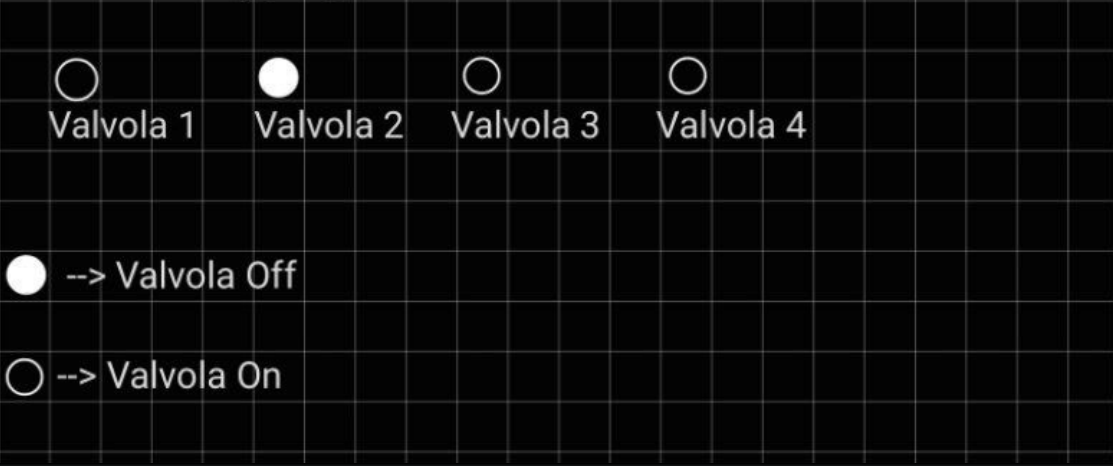
\includegraphics[width=0.8\linewidth]{img/gui_sempl.png}
    \caption{Solution 2 with simplified GUI}
  \end{subfigure}%
  \begin{subfigure}{0.5\textwidth}
    \centering
    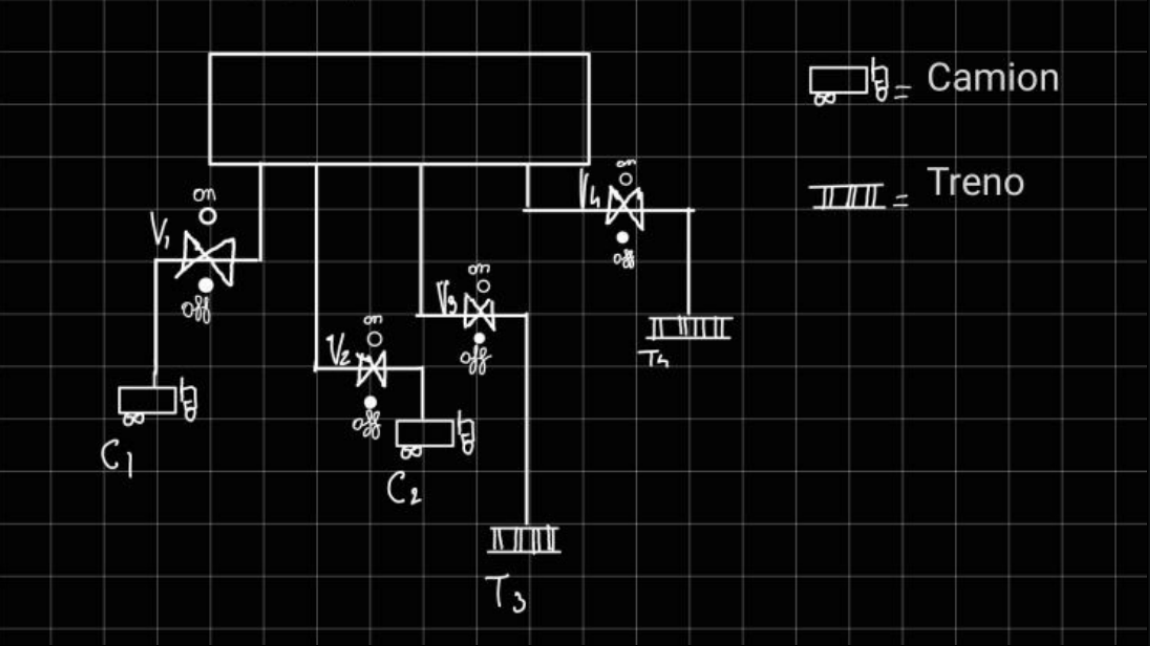
\includegraphics[width=0.8\linewidth]{img/gui_con_schema.png}
    \caption{Solution 3 GUI with system diagram}
  \end{subfigure}
  \caption{Two Solutions}
\end{figure}
\subsection{Esercizi di programmazione cli-based}
Per iniziare a creare il programma, essendo GO un linguaggio che predilige la divisione in moduli, bisogna usare il comando seguente per creare il nuovo modulo nella cartella in cui si vuole creare il file con il codice sorgente \texttt{go mod init <nome\_modulo>}.\newline 
Questo creerà un file go.mod in cui viene specificato il nome del modulo (o package) e la versione di GO:
A questo punto si può creare il file ''.go'' dove scrivere il codice sorgente.
Questo codice deve svolgere i seguenti passaggi
\begin{itemize}
\item Chiedere all'utente il numero che vuole inserire
\item Leggere il numero
\item Calcolare il fattoriale del numero inserito
\item Stampare il risultato
\end{itemize}
Nb: il linguaggio permette di inserire in un'unica istruzione gli ultimi due passaggi

\begin{lstlisting}
  
package main

import (
	"fmt"
)

func factorial(n int) int {
	if n == 0 {
		return 1
	} else {
		return n * factorial(n-1)
	}
}

func main() {
	var n int
	fmt.Println("Enter a number: ")
	fmt.Scan(&n)
	fmt.Printf("The factorial of %d is: %d ", n, factorial(n))
}
\end{lstlisting}
\begin{quote}
In questo frammento di codice, troviamo due istruzioni caratteristiche del linguaggio, ovvero:
\end{quote}
\begin{itemize}
\item package main, serve identificare dove andrà la funzione \emph{main} che serve a dare un inizio al codice.
\item  import ''fmt'', questa parte serve a dire che librerie verranno importate nel codice, fmt è la libreria standard di Go che si occupa di fornire le funzioni per elaborare I/O la sua corrispondente in C è \emph{stdio}
\end{itemize}
\subsection{Esercizi di programmazione gui-based}
Analogamente alla parte precedente, creiamo una cartella un'altra cartella di lavoro per il medesimo programma ma con una GUI, e generiamo il modulo con il comando spiegato precedentemente. Essendo una GUI più complicata da costruire, il codice sorgente sarà nettamente più lungo, infatti non useremo una libreria standard ma una libreria esterna, che si può facilmente installare attraverso il comando:
\texttt{go get github.com/gotk3/gotk3/gtk} \newline

Questo comando ''preleva'' la libreria e creerà un file go.sum usato per tenere traccia delle librerie esterne usate nel codice sorgente e aggiungerà la libreria richiesta al file go.mod. 
A questo punto si può creare il codice sorgente che svolga  le seguenti fasi:
\begin{itemize}
\item Creare una prima finestra che poi andrà riempita con le varie parti
\item Creare una griglia e un' ''etichetta'' dove andremo a mettere un'istruzione per l'utente su cosa deve fare e un'etichetta dove verrà mostrato il risultato
\item Un ''entry'' dove l'utente inserirà i numeri (NB  verranno letti come una stringa, quindi verrà convertito con la funzione Atoi())
\item Un bottone per calcolare il fattoriale del numero inserito
\item Infine ''collegare'' il bottone alla funzione effettiva per ottenere il fattoriale
\end{itemize}
NB: La libreria esterna non ha una vera e propria gestione degli errori, per questo nel codice sorgente insieme ogni dichiarazione di una variabile per creare le varie parti della GUI viene dichiarata una variabile err e viene sempre controllato che sia nulla. infatti nel caso questa variabile abbia un valore non nullo vuol dire che qualcosa è andato storto nella creazione del componente.
\begin{lstlisting}
  
  package main
  
  import (
    "fmt"
    "github.com/gotk3/gotk3/gtk"
    "log"
    "strconv"
  )
  
  func factorial(n int) int {
    if n == 0 {
      return 1
    } else {
      return n * factorial(n-1)
    }
  }
  
  func calculateFactorial(button *gtk.Button, entry *gtk.Entry, label *gtk.Label) {
    numStr, err := entry.GetText()
    if err != nil {
      log.Fatal("Error getting input:", err)
    }
  
    num, err := strconv.Atoi(numStr)
    if err != nil {
      log.Fatal("Error converting input to integer:", err)
    }
  
    result := factorial(num)
    label.SetText(fmt.Sprintf("The factorial of %d is: %d", num, result))
  }
  
  func main() {
    gtk.Init(nil)
  
    builder, err := gtk.BuilderNew()
    if err != nil {
      log.Fatal("Error initializing GTK builder:", err)
    }
  
    err = builder.AddFromFile("gui.glade")
    if err != nil {
      log.Fatal("Error loading UI file:", err)
    }
  
    obj, err := builder.GetObject("window1")
    if err != nil {
      log.Fatal("Error getting window object from UI file:", err)
    }
  
    window, ok := obj.(*gtk.Window)
    if !ok {
      log.Fatal("Error casting window object from UI file")
    }
  
    window.Connect("destroy", gtk.MainQuit)
  
    obj, err = builder.GetObject("button1")
    if err != nil {
      log.Fatal("Error getting button object from UI file:", err)
    }
  
    button, ok := obj.(*gtk.Button)
    if !ok {
      log.Fatal("Error casting button object from UI file")
    }
  
    obj, err = builder.GetObject("entry1")
    if err != nil {
      log.Fatal("Error getting entry object from UI file:", err)
    }
  
    entry, ok := obj.(*gtk.Entry)
    if !ok {
      log.Fatal("Error casting entry object from UI file")
    }
  
    obj, err = builder.GetObject("label1")
    if err != nil {
      log.Fatal("Error getting label object from UI file:", err)
    }
  
    label, ok := obj.(*gtk.Label)
    if !ok {
      log.Fatal("Error casting label object from UI file")
    }
  
    button.Connect("clicked", calculateFactorial, entry, label)
  
    window.ShowAll()
  
    gtk.Main()
  }
  \end{lstlisting}
  
\section{Guida per gli insenganti}
Per l'uso del materiale didattico fornito conviene spiegare la consegna e in seguito lasciare gli studenti ragionare su come risolvere l'esercizio. Solo dopo circa venti  minuti confrontare le soluzioni. Essendo quest'attività didattica strutturata affinché sia efficace con un apprendimento attivo si suggerisce di lasciare gli studenti ragionare tra loro e provare a dare sporadici consigli in modo che si sviluppi un ambiente di Socio-costruttivismo

Gli snodi nelle due proposte di esercizio si possono identificare icome segue nei due esercizi proposti. 
Nell'esercizio unplugged:
\begin{itemize}
\item Comprendere come collegare il comando alla singola condotta.
\item Individuare le possibili opzioni per la realizzazione dell'interfaccia, impostandone la struttura
\item Maturare un giudizio motivato su quale possa essere la soluzione più efficace dal punto di vista dell'utente
\end{itemize}

Nell'esercizio di programmazione:
\begin{itemize}
\item Comprendere la regola per il calcolo del fattoriale
\item Sviluppare il codice di base per calcolare il fattoriale
\item Comprendere come strutture una CLI 
\item Sviluppare la CLI che richiami la funzione per il calcolo del fattoriale
\item Comprendere come strutturare una GUI mediante GTK per Go
\item Sviluppare la GUI che permetta di inserire il numero di cui calcolare il fattoriale e restituirne il valore corretto
\item Maturare una valutazione critica sull'efficacia dei due approcci
\end{itemize}
\section{Valutazione}
\textbf{BLOCK MODEL}:
Una valutazione dell'esercizio di programmazione può essere basata sulla comprensione dei vari elementi del codice secondo il modello a blocchi, concentrandosi maggiormente sulle parti di "Function/Purpose".

Infatti, ai fini dell'esercizio, è importante capire il funzionamento del codice, e quindi i blocchi function/purpose e in particolare quelli relativi a block, relationship e macrostructure, mentre ai fini della valutazione dell'attività didattica i blocchi relativi alla text surface e program execution non sono rilevanti in quanto l'apprendimento dello specifico linguaggio e della sua sintassi esula dagli scopi.
Si riportano nel seguito alcune indicazioni dei blocchi da considerarsi per la strutturazione della valutazione:

Macrostructure:
Capire le funzioni principali delle tre code base del programma:
- Funzione per il calcolo del fattoriale
- Funzione per la generazione della CLI
- Funzione per la generazione della GUI

Le righe R e B si differenziano per i tre gruppi di codice:
Codice per il calcolo del fattoriale:
Relationship:
- Comprendere che il calcolo della funzione n * factorial(n-1) ripetuto ciclicamente permette di avanzare nel calcolo del fattoriale.
Blocks:
- Distinguere i due blocchi

\begin{lstlisting}
if n == 0{
    return 1
}
\end{lstlisting}

e

\begin{lstlisting}
return n*factorial(n-1)
\end{lstlisting}

distinguendone le due funzioni: il primo è l'invariante di ciclo, che arresta la ricorsione, il secondo effettua il calcolo.

Per quanto riguarda il codice per la generazione della CLI:
Relationships:
- Distinguere le parti salienti del codice: la fase di inserimento del dato e quella di elaborazione e visualizzazione del dato

Blocks:
Distinguere i 2 blocchi:

\begin{lstlisting}
var n int
fmt.Scan(&n)
\end{lstlisting}

\begin{lstlisting}
fmt.Printf("The factorial of %d is: %d",n,factorial(n))
\end{lstlisting}

Nel primo viene letto l'input dell'utente quando viene avviato il programma, nel secondo vengono stampati: il numero inserito, e il fattoriale di questo, calcolato nella funzione apposita.

Per quanto riguarda il codice per la generazione della GUI:
Relationship:
Comprendere i vari elementi che compongono la GUI (finestra, griglia, etichetta e bottone) e come legarli insieme

Blocks:
Si considerino i diversi blocchi di codice che si ripresentano in maniera similare in tutto il codice proposto, ad esempio:

\begin{lstlisting}
grid, err := gtk.GridNew()
if err != nil {
    log.Fatal("Unable to create grid:", err)
}
win.Add(grid)
\end{lstlisting}

In questa parte di codice troviamo la creazione della variabile ''grid'' che servirà a inserire specificandone la posizione i vari elementi della GUI. La variabile viene aggiunta alla finestra (variabile win) con la funzione .Attach(). Insieme a ''grid'' viene dichiarata la variabile 
''err'', che serve a gestire eventuali errori; questa gestione non deve esserci per forza nelle varie soluzioni proposte dagli studenti.

Nel secondo blocco  troviamo  il cuore dell'esercizio,infatti qui viene specificato cosa deve fare il bottone una volta cliccato, ovvero leggere il numero scritto nella casella di testo, convertirlo da stringa a intero con Atoi() e infine usare il valore come parametro della funzione per calcolare il fattoriale.
Si distinguono in maniera evidente i tre subgoal: 
\begin{itemize}
\item leggere la stringa (.GetText)
 \item convertire da stringa a intero (.Atoi)
 \item calcolare il fattoriale (factorial)
\item tampare il risultato nell'etichetta creata precedentemente (.setText)
\end{itemize}

\begin{lstlisting}
  button.Connect("clicked", func() {
  //leggere il testo dalla casella "entry"
  text, err := entry.GetText()
  if err != nil {
  log.Fatal("Unable to get text from entry:", err)
  }
  //convertire da stringa a intero
  n, err := strconv.Atoi(text)
  if err != nil {
  log.Fatal("Unable to convert text to int:", err)
  }
  //calcolare il fattoriale
  result := factorial(n)
  //stampare il risultato
  resultLabel.SetText(fmt.Sprintf("The factorial of %d is : %d ", n, result))
  })
<<<<<<< Updated upstream
\end{verbatim}
  
\textbf{POSSIBILI MISCONCEPTION}:
=======
  \end{lstlisting}
  \newpage
  \subsection{Possibili misconception}
>>>>>>> Stashed changes
  Da una ricerca su internet, emerge che per le CLI non esistono vere e proprie misconception, probabilmente perché esse tendono a essere lineari e tendono a non avere un carico cognitivo eccessivamente elevato per imparare a strutturarle.
  D'altro canto invece, si nota che le principali misconception per le GUI riguardano il design di esse, e riguardano principalmente la differenza sostanziale tra UI (User Interface) e UX (User Experience). La prima si riferisce a \textit{come} strutturare una GUI, mentre la seconda tende a studiare come migliorare al massimo l'interazione dell'utente rendendola più lineare e facile da comprendere.
  In rete sono riportate numerose misconception che riguardano il design delle UI, ossia la sua concezione in termini di organizzazione della disposizione dei comandi e della visualizzazione dei risultati, così come della sequenza delle pagine/istruzioni che possono aprirsi usufruendo della GUI stessa.
  Ulteriori misconception in termini di design riguardano l'uso dei colori, che deve sempre essere oggetto di attente valutazioni.
  Tuttavia, questo tipo di misconception non si dovrebbe manifestare in questa attività didattica, che è finalizzata a evidenziare le differenze tra CLI e GUI in termini di usabilità e di peso della programmazione.
  È comunque sicuramente opportuno che l'insegnante introduca in maniera sintetica il concetto dell'importanza di un buon design della UI e di verificarne l'usabilità con dei test su soggetti campione (test di usabilità).
  
<<<<<<< Updated upstream
\textbf{Rubrica valutativa}  
\begin{center}
  
\begin{tabular}{|p{3cm}|p{3cm}|p{3cm}|p{3cm}|p{3cm}||}
  \hline
  Campo &Incompleto & Sufficiente & Buono & Eccellente \\
  \hline
  Precisione e Organizzazione & Non si riesce a intendere bene come lo studente avrebbe voluto strutturare l'interfaccia & Lo studente ha compreso come si dovrebbe strutturare l'interfaccia ma non in maniera efficace & L'interfaccia è stata svolta correttamente, ma imprecisa in alcuni punti & L'interfaccia è stata svolta correttamente, in maniera efficace e funzionale \\
  \hline
  Interazione & La struttura disegnata/progettata non risulta per nulla intuitiva & L'interfaccia non risulta completamente intuitiva, ma comunque sufficiente per il suo utilizzo & L'interfaccia risulta intuitiva e facilmente utilizzabile ma ci sono alcuni aspetti non completamente funzionanti & L'interfaccia risulta intuitiva, facilmente utilizzabile e con tutte le funzionalità richieste \\
  \hline
  Codice & Il codice non viene presentato & Il codice viene presentato, ma risulta poco leggibile e non viene preso in considerazione l'utilizzo di metodi e di libreria esterne & Il codice viene presentato in maniera leggibile ma non viene preso in considerazione l'utilizzo di metodi e di libreria esterne & Il codice viene presentato in maniera leggibile, vengono usate le librerie e le soluzioni standard \\
  \hline
\end{tabular}

\end{center}
=======
  \subsection{Rubrica valutativa}
  \begin{center}
    \begin{tabular}{|c|p{2.5cm}|p{2.5cm}|p{2.5cm}|p{2.5cm}|}
      \hline
      & Incompleto & Sufficiente & Buono & Eccellente \\
      \hline
      Precisione e Organizzazione & Non si riesce a intendere bene come lo studente avrebbe voluto strutturare l'interfaccia & Lo studente ha compreso come si dovrebbe strutturare l'interfaccia ma non in maniera efficace & L'interfaccia è stata svolta correttamente, ma imprecisa in alcuni punti & L'interfaccia è stata svolta correttamente, in maniera efficace e funzionale \\
      \hline
      Interazione & La struttura disegnata/progettata non risulta per nulla intuitiva & L'interfaccia non risulta completamente intuitiva, ma comunque sufficiente per il suo utilizzo & L'interfaccia risulta intuitiva e facilmente utilizzabile ma ci sono alcuni aspetti non completamente funzionanti & L'interfaccia risulta intuitiva, facilmente utilizzabile e con tutte le funzionalità richieste \\
      \hline
      Codice & Il codice non viene presentato & Il codice viene presentato, ma risulta poco leggibile e non viene preso in considerazione l'utilizzo di metodi e di librerie esterne & Il codice viene presentato in maniera leggibile ma non viene preso in considerazione l'utilizzo di metodi e di libreria esterne & Il codice viene presentato in maniera leggibile, vengono usate le librerie e le soluzioni standard \\
      \hline
      Totalità & 0-5 & 6-8 & 9-12 & 13-15 \\
      \hline
    \end{tabular}
    \end{center}
>>>>>>> Stashed changes

\end{document}
